\chapter{기하학, 정보, 블랙홀 면적 법칙}

\lectureoverview{예고된 목적지는 우주론이지만, 그곳으로 가는 가장 짧은 길은 특수 상대론을 다시 살펴보는 데서 시작한다. 계량은 시공간의 기하학을 알려 주고, 고유 시간이 0이라는 조건은 빛이 어떻게 움직이는지 알려 준다. 이 규칙 하나를 슈바르츠실트 기하학에 적용하고, 지평선과 특이점을 구별한 다음, 블랙홀이 복사를 내며 사라질 때 정보가 어떻게 되는지 묻겠다. 답은 보통의 엔트로피에서 시작해 베켄슈타인의 비트 하나 논증으로 끝난다. 블랙홀은 정보를 부피가 아니라 지평선 면적 단위로 저장한다.}

서스킨드는 끈 이론의 성과와 실패를 약속한 대로 따져 보는 일을 잠시 미룬다. 늦은 시간이고, 평가보다 핵심 내용을 다루는 편이 더 유익하다고 말한다. 오늘 밤의 핵심은 블랙홀 정보 문제를 정식화하는 데 필요한 최소한의 기하학과 열역학이다.

\section{빛에 관한 하나의 규칙}

특수 상대론은 공간과 시간을 하나의 기하학적 대상으로 다룬다. 서로 \(dt,dx,dy,dz\)만큼 떨어진 이웃한 사건에 대해 서스킨드는 시간 항의 부호가 양수인 관례를 택해 다음과 같이 쓴다.
\begin{equation}
d\tau^2=dt^2-\frac{1}{c^2}\left(dx^2+dy^2+dz^2\right).
\end{equation}
시간 성분과 공간 성분의 부호가 서로 다르다는 점에서 민코프스키 기하학은 4차원 유클리드 기하학과 구별된다. 인자 \(1/c^2\)는 단위만 맞춰 준다. 시간과 거리를 일관된 단위로 측정하면 \(c=1\)로 둘 수 있다.

시간꼴 간격에서는 \(d\tau^2>0\)이고, \(d\tau\)은 그 궤적을 따라가는 시계가 기록하는 고유 시간이다. 공간꼴 간격에서는 반대로 \(d\tau^2<0\)이다. 오늘 필요한 경우는 그 두 경우의 정확한 경계에 놓인다. 빛은 \emph{널} 궤적을 따른다.
\begin{equation}
d\tau^2=0.
\end{equation}
먼저 \(x\)축 방향의 운동으로 한정하면 다음을 얻는다.
\begin{align}
0&=dt^2-\frac{dx^2}{c^2},\\
c\,dt&=\pm dx,\\
\frac{dx}{dt}&=\pm c.
\end{align}
부호는 오른쪽으로 진행하는 광선과 왼쪽으로 진행하는 광선을 나타낸다. 센티미터를 미터나 킬로미터로 바꾸면 \(c\)에 부여되는 수치가 달라진다. 불변인 진술은 수치가 아니라 널 조건이다.

일반 상대론에서는 이 규칙이 아니라 계량이 복잡해진다. 좌표가 \(x^\mu\)이고 \(\mu=0,1,2,3\)일 때,
\begin{equation}
ds^2=g_{\mu\nu}(x)\,dx^\mu dx^\nu,
\end{equation}
여기서 반복된 지표에 대해서는 합산하며, 계수는 위치에 따라 달라질 수 있다. 빛이 국소적으로 진행할 수 있는 방향을 찾으려면 이 이차 형식을 0으로 놓으면 된다.

\section{구면 좌표와 슈바르츠실트 계량}

회전하지 않는 블랙홀은 구대칭이므로, 데카르트 좌표로는 유용한 구조가 잘 드러나지 않는다. \(r\)를 반지름 방향 거리로, \(\theta,\phi\)를 단위 구면 위의 방향을 나타내는 좌표로 두자. 구면의 선요소는 다음과 같다.
\begin{equation}
d\Omega^2=d\theta^2+\sin^2\theta\,d\phi^2.
\end{equation}
반지름이 \(r\)인 구면에서는 각방향 변위가 따라서 \(r^2d\Omega^2\)만큼 기여한다. 구면 좌표로 쓴 평탄한 시공간은 다음과 같다.
\begin{equation}
d\tau^2=dt^2-\left(dr^2+r^2d\Omega^2\right),
\qquad (c=1).
\end{equation}

서스킨드는 아인슈타인 방정식에서 블랙홀 해를 유도하지 않는다. 식을 적어 놓고 살펴보자고 한다. 칠판에는 비교하려는 대상이 명확히 드러나 있다.

\begin{figure}[htbp]
\centering
\includegraphics[width=0.86\textwidth]{lecture_02_figure_02.png}
\caption{위쪽에는 평탄한 구면 시공간, 아래쪽에는 슈바르츠실트 변형이 그려져 있다. 반복되는 인자 \(1-2GM/(c^2r)=1-R_s/r\)와 반지름 방향 스케치가 함께 보인다.}
\lectureframe{00:19:12.520}
\end{figure}

질량이 \(M\)인 블랙홀에 대해 슈바르츠실트 반지름을 다음과 같이 정의하자.
\begin{equation}
R_s=\frac{2GM}{c^2}.
\end{equation}
외부 영역의 선요소는 다음과 같다.
\begin{equation}
d\tau^2=\left(1-\frac{R_s}{r}\right)dt^2
-\frac{dr^2/c^2}{1-R_s/r}
-\frac{r^2}{c^2}d\Omega^2.
\label{eq:schwarzschild-explicit-c}
\end{equation}
동등하게, \(c=1\)로 두면 다음과 같이 쓸 수 있다.
\begin{equation}
ds^2=\left(1-\frac{2GM}{r}\right)dt^2
-\frac{dr^2}{1-2GM/r}-r^2d\Omega^2.
\label{eq:schwarzschild}
\end{equation}
멀리 떨어진 곳에서는 \(R_s/r\ll1\)이므로 평탄한 구면 계량으로 돌아간다. 이 점근적 검산은 공식을 외우는 것보다 중요하다. 그래도 서스킨드는 칵테일 파티에서 이야기할 거리로 공식을 외워 두라고 권한다.

\editorialnote{칠판에서는 \(d\tau^2\)와 \(ds^2\)를 번갈아 쓰며, 인자 \(c\)를 일관되게 모두 표시하지는 않는다. 식~\eqref{eq:schwarzschild-explicit-c}은 시간 좌표에 관한 강의의 관례를 따르며, 이때 \(t\)의 단위는 시간이다. \(x^0=ct\)를 쓰는 표준형도 대수적으로 동등하다.}

\subsection{지평선은 특이점이 아니다}

좌표상 두 반지름에서 이상한 점이 보인다. 자연 단위계에서 \(r=R_s=2GM\)일 때 \(dt^2\)의 계수는 사라지고 \(dr^2\)의 계수는 발산한다. \(r=0\)에서는 곡률 자체가 특이해진다. 이는 같은 현상의 두 가지 표현이 아니다:
\begin{equation}
\begin{aligned}
r=R_s &:\quad \text{horizon},\\
r=0 &:\quad \text{curvature singularity}.
\end{aligned}
\end{equation}

조석력으로 두 경우의 물리적 차이를 알 수 있다. 중력장은 크기가 있는 물체의 위치에 따라 달라진다. 발이 머리보다 더 큰 힘을 받아 몸이 늘어나고, 가로 방향은 압축될 수 있다. 지평선에서 조석력은 유한하며, 충분히 무거운 블랙홀의 지평선에서는 아주 작을 수도 있다. 그곳에서 국소적으로 재앙적인 일이 반드시 일어나는 것은 아니다. 반면 \(r=0\)에서는 조석력이 발산한다. \(r=R_s\)에서 나타나는 문제의 계수는 슈바르츠실트 좌표의 결함을 나타내지만, \(r=0\)의 특이점은 물리적인 특이점이다.

\editorialnote{곡률이 \(r=R_s\)에서 유한하다는 점은 크레치만 스칼라 \(R_{\mu\nu\rho\sigma}R^{\mu\nu\rho\sigma}=48G^2M^2/(c^4r^6)\)로 확인할 수 있다. 이 값은 지평선에서 유한하고 \(r\to0\)일 때만 발산한다. 이 불변량은 강의 중 칠판에 쓰이지 않았지만, 조석력에 관한 구별을 정확히 해 준다.}

\section{지평선 부근의 방사형 광선}

이제 하나의 규칙으로 돌아가자. 방사형 광선은 각좌표를 고정한 채 진행하므로 \(d\Omega=0\)이고, 빛의 광선은 \(ds^2=0\)이다. \(c=1\) 단위계에서 식~\eqref{eq:schwarzschild}은 다음을 준다.
\begin{equation}
0=\left(1-\frac{2GM}{r}\right)dt^2
-\frac{dr^2}{1-2GM/r}.
\end{equation}
양변에 \(1-2GM/r\)를 곱하고 제곱근을 취하면 두 갈래가 나온다.
\begin{align}
dr&=\pm\left(1-\frac{2GM}{r}\right)dt,\\
\frac{dr}{dt}&=\pm\left(1-\frac{2GM}{r}\right).
\label{eq:radial-null}
\end{align}
양의 부호는 바깥쪽으로 나가는 광선, 음의 부호는 안쪽으로 들어가는 광선을 나타낸다. 멀리 떨어진 곳에서는 이들의 좌표 속도가 \(\pm1\)에 가까워진다. 지평선에서는 두 경우 모두 \(\lvert dr/dt\rvert\to0\)를 만족한다. 슈바르츠실트 좌표 시간으로 보면 바깥쪽 광선은 그곳에서 정지한 것처럼 보이고, 안쪽 광선은 도달하는 데 무한한 좌표 시간이 걸린다.

\begin{figure}[htbp]
\centering
\includegraphics[width=0.82\textwidth]{lecture_02_figure_03.png}
\caption{완성된 \(t\)-\(r\) 칠판 스케치. 점선 지평선에 가까워질수록 방사형 널 광선은 수직에 가까워진다.}
\lectureframe{00:30:25.000}
\end{figure}

\begin{figure}[htbp]
\centering
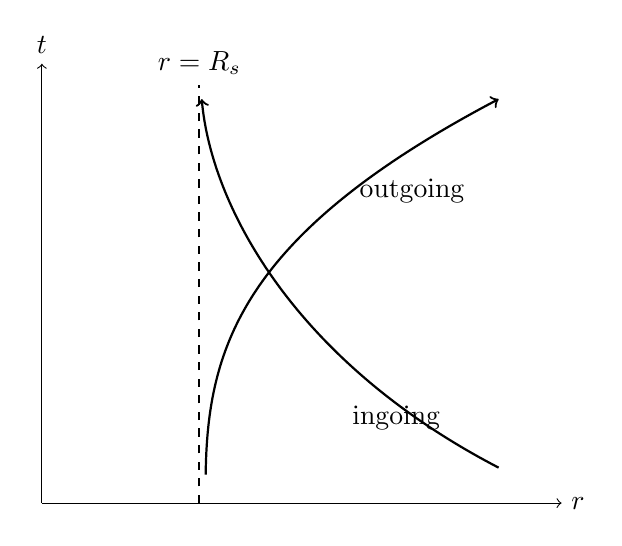
\begin{tikzpicture}[x=1.0cm,y=0.9cm]
\draw[->] (0,0) -- (6.6,0) node[right] {$r$};
\draw[->] (0,0) -- (0,6.2) node[above] {$t$};
\draw[dashed,thick] (2.0,0) -- (2.0,5.9) node[above] {$r=R_s$};
\draw[thick,->] (2.08,.4) .. controls (2.10,2.2) and (2.55,3.8) .. (5.8,5.7);
\draw[thick,->] (5.8,.5) .. controls (3.2,2.0) and (2.15,4.2) .. (2.03,5.7);
\node[align=center] at (4.7,4.4) {outgoing};
\node[align=center] at (4.5,1.2) {ingoing};
\end{tikzpicture}
\caption{좌표 시간을 기준으로 정리한 칠판 스케치. 느려지는 듯한 현상은 슈바르츠실트 좌표의 \(t\)에 관한 진술이지, 빛이 국소적으로 \(c\)로 움직이지 않는다는 뜻은 아니다.}
\end{figure}

지평선 안쪽에서는 미래 방향 광선뿔이 안쪽으로 크게 기울어져, 미래 방향의 방사형 광선 두 갈래 모두 \(r\)가 감소하는 방향으로 향한다. 그곳에서 시작된 신호는 외부로 탈출할 수 없으며, 미래 방향의 모든 인과적 경로는 특이점에 도달한다.

\begin{classroomqa}\audiencequestion{빛의 속도가 불변이라면, 지평선 부근에서 빛이 느려진다고 말하는 것은 정확히 무슨 뜻인가요?\lecturetimestamp{00:31:44}}\lecturerresponse{표시된 양은 특정 좌표계에서의 \(dr/dt\)이다. 미터를 센티미터로 바꾸기만 해도 수치상의 속도는 달라진다. 여기서는 위치에 따라 유효한 반지름 방향 눈금과 시간 눈금이 달라진다. 보편적으로 성립하는 진술은 모든 빛의 광선이 널 궤적 \(ds^2=0\)을 따른다는 것이다.}\end{classroomqa}\editorialnote{자유 낙하하는 국소 관측자는 진공에서 빛의 속도를 \(c\)로 측정한다. 지평선에서 슈바르츠실트 좌표 속도가 사라지는 현상은 국소 관측량이 아니다.}

\begin{classroomqa}\audiencequestion{빛이 통과하는 물질 매질과 관계없이 같은 널 속도 진술이 성립하나요?\lecturetimestamp{00:33:24}}\lecturerresponse{아니요. 남아 있는 기록으로는 이 답변에 관해 더 긴 설명을 확인할 수 없다.}\end{classroomqa}\editorialnote{널 속도에 관한 주장은 진공 시공간에서의 전파를 다룬다. 물질과의 상호작용으로 파동 묶음의 유효 속도가 더 작아질 수 있다. 이것은 매질의 특성이지, 국소적인 인과 속도 \(c\)가 바뀌는 것은 아니다.}

\begin{classroomqa}\audiencequestion{같은 \(t\)-\(r\) 도표에서 안쪽으로 들어오는 광선은 어떻게 보이나요?\lecturetimestamp{00:33:32}}\lecturerresponse{반대 방향으로 보이는 갈래다. 큰 \(r\)에서 출발해 지평선 쪽으로 휘어지며 점근적으로 가까워진다. 도달하는 데 좌표 시간 \(t\)이 무한히 걸린다.}\end{classroomqa}\editorialnote{낙하하는 관측자는 유한한 고유 시간 안에 지평선에 도달해 통과한다. 발산하는 것은 슈바르츠실트 좌표의 \(t\)뿐이다.}

\section{증발이 문제를 일으키는 이유}

지평선은 훨씬 더 깊이 살펴볼 만한 주제다. 어떻게 형성되는지, 낙하하는 관측자가 무엇을 보는지, 그곳에서 국소적으로 특이한 일이 일어나는지 등을 알아야 한다. 서스킨드는 그런 질문은 미뤄 두고 양자역학으로 넘어간다. 외부에서 보면 물질과 그 물질을 구별해 주는 모든 정보가 지평선에 점점 더 가까이 압축되어 접근할 수 없게 된다. 그렇다고 해서 정보가 파괴되는 것은 아니다. 단지 숨겨졌을 수 있다.

호킹의 결과는 이 문제를 첨예하게 만든다. 안정된 고전적 블랙홀은 상상할 수 있는 가장 무미건조한 물체처럼 보인다. 구형이고 어두우며 메시지를 보낼 수 없다. 하지만 ``검다''는 두 가지 뜻을 갖는다. 아무것도 방출하지 않는다는 뜻일 수도 있고, 열적 흑체 복사를 방출한다는 뜻일 수도 있다. 양자 블랙홀은 두 번째 의미에서 검다. 온도가 있고 빛을 내며 에너지를 잃는다. 다음 관계에 따라
\begin{equation}
E=Mc^2,
\qquad
R_s=\frac{2GM}{c^2},
\end{equation}
복사는 질량과 지평선 반지름을 모두 감소시킨다. 증발이 결국 블랙홀을 없애 버린다면, 지평선에 남아 있는 듯했던 정보는 어떻게 될까? 정보가 파괴될 수도 있고, 작은 잔해에 갇힐 수도 있으며, 바깥으로 나가는 복사에 부호화될 수도 있다. 이런 가능성 사이의 긴장이 바로 정보 문제이며, 뒤에서 끈 이론이 그 해법을 더 분명히 하는 데 도움을 줄 것이다.

오늘 밤에는 곡률 시공간에서의 양자장 계산을 시도하지 않는다. 대신 서스킨드는 베켄슈타인의 더 간단한 접근을 따른다. 먼저 엔트로피를 정보로 이해하고, 이어서 블랙홀이 얼마나 많은 정보를 숨길 수 있는지 계산한다.

\section{존재하지만 숨겨진 정보}

상자를 칸으로 나눈다고 하자. 각 칸은 충분히 작아서 비어 있거나 차 있는 둘 중 하나다. 이진 문자열------은 각 칸에 대해 하나씩 답을 주며, 그 배치가 허용된 다른 모든 배치와 구별되도록 한다. 더 현실적인 물질에서는 입자 종류와 다른 자유도에 관한 질문도 필요하지만, 원리는 같다. 정보는 상태를 지정하는 데 필요한 최소한의 예--아니요 질문의 수로 측정한다.

\begin{classroomqa}\audiencequestion{이것은 정적인 계를 설명하는 것에 불과한가요?\lecturetimestamp{00:45:49}}\lecturerresponse{한 순간의 상태를 기술하는 순간적인 설명이다. 그다음 동역학이 그 상태를 다른 상태로 변환한다.}\end{classroomqa}

다음 원리는 더 근본적이다. 닫힌 계의 시간 진화는 서로 다른 두 미시 상태를 하나로 합치지 않는다. 지금 서로 다른 두 배치는 시간에 따라 변한 뒤에도 원칙상 구별할 수 있다. 고전적인 해밀턴 시간 진화는 가역적이고, 양자 시간 진화는 유니터리다.\editorialnote{소산적인 유효 방정식이 구별을 지울 수 있는 것은 관측하지 않은 환경의 자유도를 생략했기 때문이다. 완전한 닫힌 계의 상태에는 그 구별이 남아 있다.}

욕조의 예를 보면 정보의 소실과 접근 불가능성의 차이가 구체적으로 드러난다. 물방울이 흐르는 두 가지 방식에 서로 다른 모스 부호 메시지를 담을 수 있다. 물이 잔잔해지고 나면 두 욕조는 똑같아 보인다. 눈에 보이는 잔물결은 사라졌지만, 미시 상태를 완전히 측정하면 분자 배치가 서로 다르다는 것을 여전히 알아낼 수 있다. 메시지는 추적하기에는 너무 작고 수가 많은 자유도로 퍼져 나갔다.

엔트로피는 이렇게 숨겨진 정보다. 우리가 던질 수 있는 거시적 질문---온도, 총에너지, 조성, 물 높이---을 기준으로 보면, 가능한 미시적 차이는 많이 남아 있지만 접근할 수 없다. 강의에서 사용한 비트 세기 표현으로는 다음과 같다.
\begin{equation}
S=\hbox{number of hidden bits}.
\end{equation}
정확한 통계역학 공식은 \(S=k_B\ln\Omega\)이지만, 블랙홀 논증에는 정성적인 정의만으로 충분하다.

\section{비트를 숨기는 비용으로서의 온도}

온도는 측정하기에는 익숙하지만, 정의는 놀라울 만큼 간접적이다. 서스킨드는 엔트로피와 에너지를 기본 개념으로 삼는다. 컴퓨터 비트를 표준값으로 재설정한다고 하자. 물리적 장치는 그대로 있지만, 컴퓨터 안에서는 이전의 0 상태와 1 상태의 구별이 사라진다. 그 구별이 완전한 세계에서 사라질 수는 없다. 환경의 미시적 자유도로 옮겨 가며, 환경은 조금 가열된다. 이것이 란다우어 원리다.

엔트로피 단위를 비트 하나로 삼고 온도를 에너지 단위로 측정하면, 강의에서는 다음과 같이 쓴다.
\begin{align}
\Delta S&=1,\\
\Delta E&=T\,\Delta S,\\
dE&=T\,dS.
\label{eq:first-law}
\end{align}

\begin{figure}[htbp]
\centering
\includegraphics[width=0.84\textwidth]{lecture_02_figure_04.png}
\caption{칠판에 적힌 정보 이론적 열역학. \(S\)는 엔트로피이고, 숨겨진 비트 하나는 \(\Delta S=1\)를 가지며, 그 최소 에너지 비용은 \(\Delta E=T\Delta S\)로 쓴다.}
\lectureframe{00:58:40.000}
\end{figure}

\editorialnote{통상적인 단위계에서 이진 비트 하나를 가역적으로 지우는 데 드는 비용은 \(k_BT\ln2\)이다. 식~\eqref{eq:first-law}에서는 \(k_B=1\)로 두고, 강의의 엔트로피 단위를 비트 하나로 취하면서 이에 따르는 \(\ln2\)를 생략한다. 이러한 관례는 이어지는 스케일링 논증에 영향을 주지 않는다.}

청중의 한 추산에 따르면, 대략 \(100\) 기가바이트를 지울 때 물 한 잔의 온도 상승은 최저 \(10^{-15}\)도 정도다. 서스킨드는 정확한 수치보다 요점을 받아들인다. 실온에서 비트 하나가 갖는 최소 에너지는 극도로 작으며, 실제 컴퓨터는 소거를 가역적으로 하지 않기 때문에 훨씬 더 많은 에너지를 열로 방출한다.

\begin{classroomqa}\audiencequestion{하드 드라이브의 예는 비유에 불과한가요, 아니면 소거에 따른 가열도 실제 법칙인가요?\lecturetimestamp{01:00:02}}\lecturerresponse{실제 물리적 제약이며, 란다우어 법칙이다. 메모리 셀을 재설정하면 컴퓨터에서 기존의 구별이 없어지므로, 그 정보는 환경으로 전달되어야 한다. 일반적인 연산은 회로를 구동하고 전하를 이동시키며 무관한 열도 발생시키므로, 이상적인 최소 비용보다 훨씬 비효율적이다.}\end{classroomqa}

\begin{classroomqa}\audiencequestion{더 높은 온도에서는 비트 하나를 숨기는 데 더 많은 에너지가 드나요?\lecturetimestamp{01:02:07}}\lecturerresponse{그렇다. 관계식 \(dE=T\,dS\)가 바로 이를 말한다. 같은 엔트로피를 전달하더라도 더 뜨거운 열저장고에서는 더 많은 에너지가 전달되어야 한다. 에너지와 숨겨진 비트 사이의 이 관계를 온도의 정의로 보아도 된다.}\end{classroomqa}

\begin{classroomqa}\audiencequestion{이미 저장된 비트 위에 새 정보를 덮어쓰면 기존 정보는 사라진 건가요?\lecturetimestamp{01:02:43}}\lecturerresponse{컴퓨터에서는 사라졌지만, 닫힌 물리계에서는 사라지지 않았다. 덮어쓴 구별은 환경으로 퍼져 나갔으며, 그곳에서 접근 불가능한 정보에 기여하므로 엔트로피를 증가시킨다.}\end{classroomqa}

열역학적 엔트로피를 누락된 미시 정보와 동일시하는 생각은 볼츠만까지 거슬러 올라간다. 섀넌은 20세기에 이에 대응하는 정보 이론의 언어를 제시했다. 서스킨드는 자신과 청중 일부가 들었던 1950년대의 열역학 강의에서는 이런 설명이 이상할 만큼 빠져 있었다고 말한다. 컴퓨터 과학은 이 연결을 지나치기 어렵게 만들었지만, 그 물리적 내용을 처음 제시한 것은 아니다.

\section{블랙홀에 비트 하나 넣기}

욕조를 물방울 하나씩 채우듯, 블랙홀도 개념적으로 비트 하나씩 만들어 볼 수 있다. 질문은 미분적이다. 정보를 하나 더 숨기면 지평선은 얼마나 커지는가? 질량이 \(M\)이고 반지름이 \(R_s\)인 블랙홀에서 시작해, 흡수되었는지 여부만 복원 가능한 구별로 갖는 가장 단순한 물체를 안으로 보낸다.

\begin{classroomqa}\audiencequestion{정보가 블랙홀 안으로 들어가는 데 좌표 시간이 무한히 걸리지 않나요?\lecturetimestamp{01:08:07}}\lecturerresponse{정보는 지평선 부근에서 지수적으로 압축되어 짧은 실용적 시간 안에 외부에서 접근할 수 없게 된다. 실제로 지평선을 통과하는 데 슈바르츠실트 좌표 시간으로 무한대가 주어지더라도 그렇다. 따라서 외부에서 하는 셈에서는 그 정보가 지평선에 저장되었다고 볼 수 있다.}\end{classroomqa}

광자는 자연스러운 후보지만, 일반적인 광자는 비트 하나보다 많은 정보를 갖는다. 편광은 이진 선택을 부호화할 수 있다. 도착 위치를 정밀하게 국소화하면 위쪽 반구인지 아래쪽 반구인지, 왼쪽 절반인지 오른쪽 절반인지 등 많은 예--아니요 질문이 추가된다. 양자역학은 국소화 정도를 대략 파장으로 제한하므로, 위치 정보를 억제하려면 블랙홀이 흡수할 수 있는 가장 긴 파장을 사용해야 한다.

\begin{classroomqa}\audiencequestion{광자가 그보다 더 긴 파장을 가지면 블랙홀에 들어갈 수 없는 상한이 정말 있나요?\lecturetimestamp{01:12:15}}\lecturerresponse{그렇다. 블랙홀보다 훨씬 큰 파동은 주로 흡수되지 않고 산란된다. 경계에 가까운 유용한 선택은 지평선 반지름에 맞먹는 파장이다. 입사 지점을 흐릿하게 할 만큼 길면서도 흡수 확률이 상당할 만큼 짧다.}\end{classroomqa}

\begin{classroomqa}\audiencequestion{광자가 어느 방향에서 오는지도 그 자체로 정보를 더하지 않나요?\lecturetimestamp{01:13:28}}\lecturerresponse{파장이 지평선 전체 크기 정도라면 장은 블랙홀을 가로질러 아주 천천히 변하므로, 입사 방향을 정밀하게 구분할 수 없다. 이 때문에 장파장 극한에서는 정밀하게 위치가 정해진 충돌이 아니라 하나의 예--아니요 정보만 근사적으로 다루게 된다.}\end{classroomqa}

따라서 크기 차수로 다음과 같이 택하자.
\begin{equation}
\lambda\sim R_s=\frac{2GM}{c^2}.
\label{eq:one-bit-wave}
\end{equation}
광자의 운동학으로부터 다음을 얻는다.
\begin{equation}
E=cp,
\qquad
p=\hbar k=\frac{h}{\lambda},
\qquad
\Delta E\sim\frac{\hbar c}{R_s}.
\label{eq:one-bit-energy}
\end{equation}
여기서는 \(k=2\pi/\lambda\)이고 \(h=2\pi\hbar\)이다. 강의에서는 \(2\pi\)를 의도적으로 무시하며, 흡수에 따르는 1 정도의 인자도 생략한다.

\begin{classroomqa}\audiencequestion{운동량을 \(\hbar/\lambda\)로 써야 하나요, 아니면 \(h/\lambda\)로 써야 하나요?\lecturetimestamp{01:16:00}}\lecturerresponse{보통 파장을 뜻하는 \(\lambda\)를 쓰면 정확한 관계는 \(p=h/\lambda=2\pi\hbar/\lambda\)이고, 파수를 뜻하는 \(k=2\pi/\lambda\)를 쓰면 \(p=\hbar k\)이다. 여기서의 추산은 스케일만 남기므로 인자 \(2\pi\)는 의도적으로 버린다.}\end{classroomqa}

비트 하나를 숨기는 데 드는 에너지가 온도의 스케일이다. 따라서 식~\eqref{eq:one-bit-wave}과 식~\eqref{eq:one-bit-energy}에서 다음을 얻는다.
\begin{equation}
k_BT_H\sim\frac{\hbar c}{R_s}
\sim\frac{\hbar c^3}{GM}.
\end{equation}
정확한 호킹 결과는 다음과 같다.
\begin{equation}
k_BT_H=\frac{\hbar c^3}{8\pi GM}.
\end{equation}
기초적인 논증은 \(M,G,c,\hbar\)에 대한 의존성은 구하지만 계수는 구하지 못한다.

\section{비트 하나는 플랑크 스케일 패치 하나를 차지한다}

같은 광자로 지평선이 얼마나 커지는지도 알 수 있다. 광자의 에너지는 질량을 다음만큼 변화시킨다.
\begin{equation}
\Delta M=\frac{\Delta E}{c^2}
\sim\frac{\hbar}{cR_s}.
\end{equation}
\(R_s=2GM/c^2\)이므로,
\begin{equation}
\Delta R_s=\frac{2G}{c^2}\Delta M
\sim\frac{G\hbar}{c^3R_s},
\end{equation}
여기서도 1 정도인 인자는 모두 생략했다. \(R_s\)를 곱하면,
\begin{equation}
R_s\Delta R_s\sim\frac{G\hbar}{c^3}.
\end{equation}
\(A=4\pi R_s^2\)이므로 그 미분은 \(dA=8\pi R_s\,dR_s\)이다. 따라서
\begin{equation}
\Delta A\sim\frac{G\hbar}{c^3}=\ell_P^2,
\qquad
\ell_P=\sqrt{\frac{G\hbar}{c^3}}.
\label{eq:planck-patch}
\end{equation}

\begin{figure}[htbp]
\centering
\includegraphics[width=0.84\textwidth]{lecture_02_figure_05.png}
\caption{칠판에서 스케일링 논증이 완성되었다. 1비트의 에너지 \(\Delta E\sim\hbar c/R_s\)는 반지름의 제곱, 따라서 면적이 \(G\hbar/c^3\) 정도 증가함을 뜻한다.}
\lectureframe{01:22:40.000}
\end{figure}

칠판에서 계산을 진행하는 동안 인자 \(c\)를 계산 중간에 복원하자, 청중 한 명이 슈바르츠실트 반지름에서 빠진 \(c^{-2}\)를 지적한다. 바로 그 수정으로 식~\eqref{eq:planck-patch}의 \(c^{-3}\)가 나온다.

\begin{classroomqa}\audiencequestion{계산의 일부에서만 \(c\)를 복원하면서 그 인자의 제곱이 누락된 건가요?\lecturetimestamp{01:21:18}}\lecturerresponse{그렇다. 차원 관계는 \(R_s=2GM/c^2\)이지 단순히 \(2GM\)가 아니다. 이 인자를 복원하면 면적의 스케일은 \(G\hbar/c^3\)가 된다.}\end{classroomqa}

\(G\simeq6.7\times10^{-11}\,\mathrm{m^3\,kg^{-1}\,s^{-2}}\), \(\hbar\simeq1.05\times10^{-34}\,\mathrm{J\,s}\), \(c^3\simeq2.7\times10^{25}\,\mathrm{m^3\,s^{-3}}\)를 사용하면,
\begin{equation}
\ell_P^2\simeq2.6\times10^{-70}\,\mathrm{m^2},
\qquad
\ell_P\simeq1.6\times10^{-35}\,\mathrm{m}.
\end{equation}
칠판에서 추산하는 동안 강의에서 말로 언급한 지수는 오락가락하지만 물리적 결론은 변하지 않는다. 이 스케일은 직접 측정으로 분해할 수 있는 한계보다 훨씬 작다.

기억에 남는 비유는 뾰족한 팔꿈치를 가진 꿰뚫을 수 없는 비트들이 지평선에 쌓이며 서로를 밀어내는 모습이다. 새 비트 하나가 대략 플랑크 면적 패치 하나를 차지한다. 이것은 면적을 셈하는 방식을 설명하는 비유이지, 지평선이 문자 그대로 정사각형 타일로 이루어져 있다는 주장이 아니다.

\begin{classroomqa}\audiencequestion{첫 광자가 아직 다가오는 중에 다른 광자가 지평선을 키우면, 앞서 온 광자는 새 지평선 안에 있게 되는 것 아닌가요?\lecturetimestamp{01:26:39}}\lecturerresponse{단순한 정적 그림만으로는 이 질문에 정확히 답할 수 없다. 동적 시공간의 사건 지평선은 전역적으로 정의해야 하며, 물질이 들어오면서 그 위치도 바뀐다. 여기서 사용한 외부 관점에서는 정보가 커지는 지평선과 계속 연관되어 있다. 지평선을 신중히 정의하는 일은 뒤로 미룬다.}\end{classroomqa}

\begin{classroomqa}\audiencequestion{예를 들어 두 블랙홀이 충돌할 때처럼 큰 질량을 더해도 같은 문제가 생기나요?\lecturetimestamp{01:27:03}}\lecturerresponse{그렇다. 이때는 동역학적 성격을 무시할 수 없다. 강의에서는 지평선을 더 신중히 정의할 때까지 병합의 전체 기하학을 다루지 않는다.}\end{classroomqa}

\begin{classroomqa}\audiencequestion{플랑크 면적은 구면 지평선 위가 아니라 평평한 패치에만 정의되나요?\lecturetimestamp{01:27:30}}\lecturerresponse{플랑크 면적은 구면의 곡면 위에 놓인 면적 스케일이며, 지평선이 평평해야 한다는 뜻은 아니다. 이 셈에서는 평면과 구면의 차이가 중요하지 않다.}\end{classroomqa}\editorialnote{지평선의 곡률 반지름이 \(\ell_P\)보다 훨씬 크면 플랑크 크기의 각 영역은 국소적으로 거의 평평하다.}

지름이 8킬로미터인 블랙홀이라면, 경계에 해당하는 광자는 그 정도 길이의 긴 전파가 된다. 청중은 물체의 크기와 무관한 면적 증가량을 설명하려고, 농구공이나 지구를 감은 끈에 같은 길이의 둘레를 더하는 비유를 든다. 어느 경우든 고정된 둘레 증가로 생기는 반지름 방향 간격은 같다. 두 예의 정확한 기하학은 다르지만, 각각 물체의 원래 크기와 무관한 변화를 보여 준다.

\section{면적 법칙}

비트를 하나씩 더할 때마다 지평선 면적은 보편적인 미시적 양만큼 변한다. 따라서 숨길 수 있는 비트의 수는 부피가 아니라 \(A/\ell_P^2\)에 비례해야 한다. 베켄슈타인은 비례 관계를 추론했고, 호킹의 계산으로 그 계수가 정해졌다.
\begin{equation}
S_{\mathrm{BH}}=\frac{k_B A c^3}{4G\hbar}
=\frac{k_B A}{4\ell_P^2}.
\label{eq:bh-entropy}
\end{equation}
엔트로피를 열역학적 단위가 아니라 이진 비트로 세려면 \(S_{\mathrm{BH}}/k_B\)을 \(\ln2\)로 나누면 된다.

\begin{figure}[htbp]
\centering
\includegraphics[width=0.84\textwidth]{lecture_02_figure_06.png}
\caption{호킹의 계수 \(1/4\)를 포함한 칠판의 최종 공식이다. 강의에서 사용하는 엔트로피 단위로는 \(S\propto Ac^3/(4G\hbar)\)이다.}
\lectureframe{01:31:02.000}
\end{figure}

따라서 블랙홀은 크기가 비슷한 보통의 계보다 엔트로피가 훨씬 크다. 그래도 그 값은 순진하게 부피를 기준으로 셈했을 때 예상할 수 있는 것보다는 작다. 서로 독립적인 정보의 양은 표면량으로 제한된다. 이 역전---정보가 2차원 경계의 스케일을 따라 변하는 양으로 3차원 중력 영역을 기술한다는 점---이 홀로그래피 원리의 씨앗이다.

\begin{classroomqa}\audiencequestion{엔트로피 공식의 인자 \(1/4\)는 어디서 나오나요?\lecturetimestamp{01:30:30}}\lecturerresponse{베켄슈타인의 논증은 면적과 기본 상수에 대한 의존성을 정했지만 계수는 미지수로 남겼다. 그의 추산에서는 2의 로그 같은 값도 후보로 나왔다. 호킹의 양자장 계산으로 계수는 정확히 \(1/4\)로 정해졌다.}\end{classroomqa}

\(\hbar\)의 위치에 마지막 놀라움이 담겨 있다. 양자 엔트로피는 \(\hbar\)에 비례해 고전적 극한에서 사라질 것으로 예상할 수 있다. 하지만 실제로는 \(\hbar\)가 분모에 놓인다. \(\hbar\to0\)일 때 파동은 임의로 작은 에너지 비용으로 임의로 세밀한 정보를 담을 수 있으므로, 엔트로피 용량은 발산한다. 양자화는 본질적으로 고전적인 블랙홀에 작은 엔트로피를 더하는 것이 아니라, 정보 용량이 무한대가 되는 것을 막는다.

\begin{classroomqa}\audiencequestion{각운동량의 단위인 \(\hbar\)가 보통의 운동량과 파장 사이의 관계도 정하는 이유는 무엇인가요?\lecturetimestamp{01:33:23}}\lecturerresponse{\(\hbar\)는 작용의 단위를 가지며, 이는 운동량과 거리의 곱과 같다. \(p\lambda\)도 같은 단위이므로, 양자 관계는 \(2\pi\) 관례를 제외하면 \(p\sim\hbar/\lambda\)로 쓸 수 있다. 각운동량 \(\mathbf r\times\mathbf p\)도 같은 이유로 같은 차원을 갖는다.}\end{classroomqa}

강의는 여기서 멈춘다. 주제가 끝났기 때문이 아니라, 지금이 적절한 경계이기 때문이다. 기하학은 지평선이 왜 정보를 숨기는지 알려 주었고, 열역학은 숨겨진 정보를 어떻게 셀지 알려 주었으며, 양자역학은 비트 하나당 유한한 면적을 제시했다. 이제 다음 질문은 블랙홀에 미시 상태가 있는지가 아니라, 그 상태가 낙하한 정보를 어떻게 부호화하고 결국 되돌려 주는지다.